\section{Introduction}
\label{sec:intro}

\begin{figure}[!t]
	\centering
	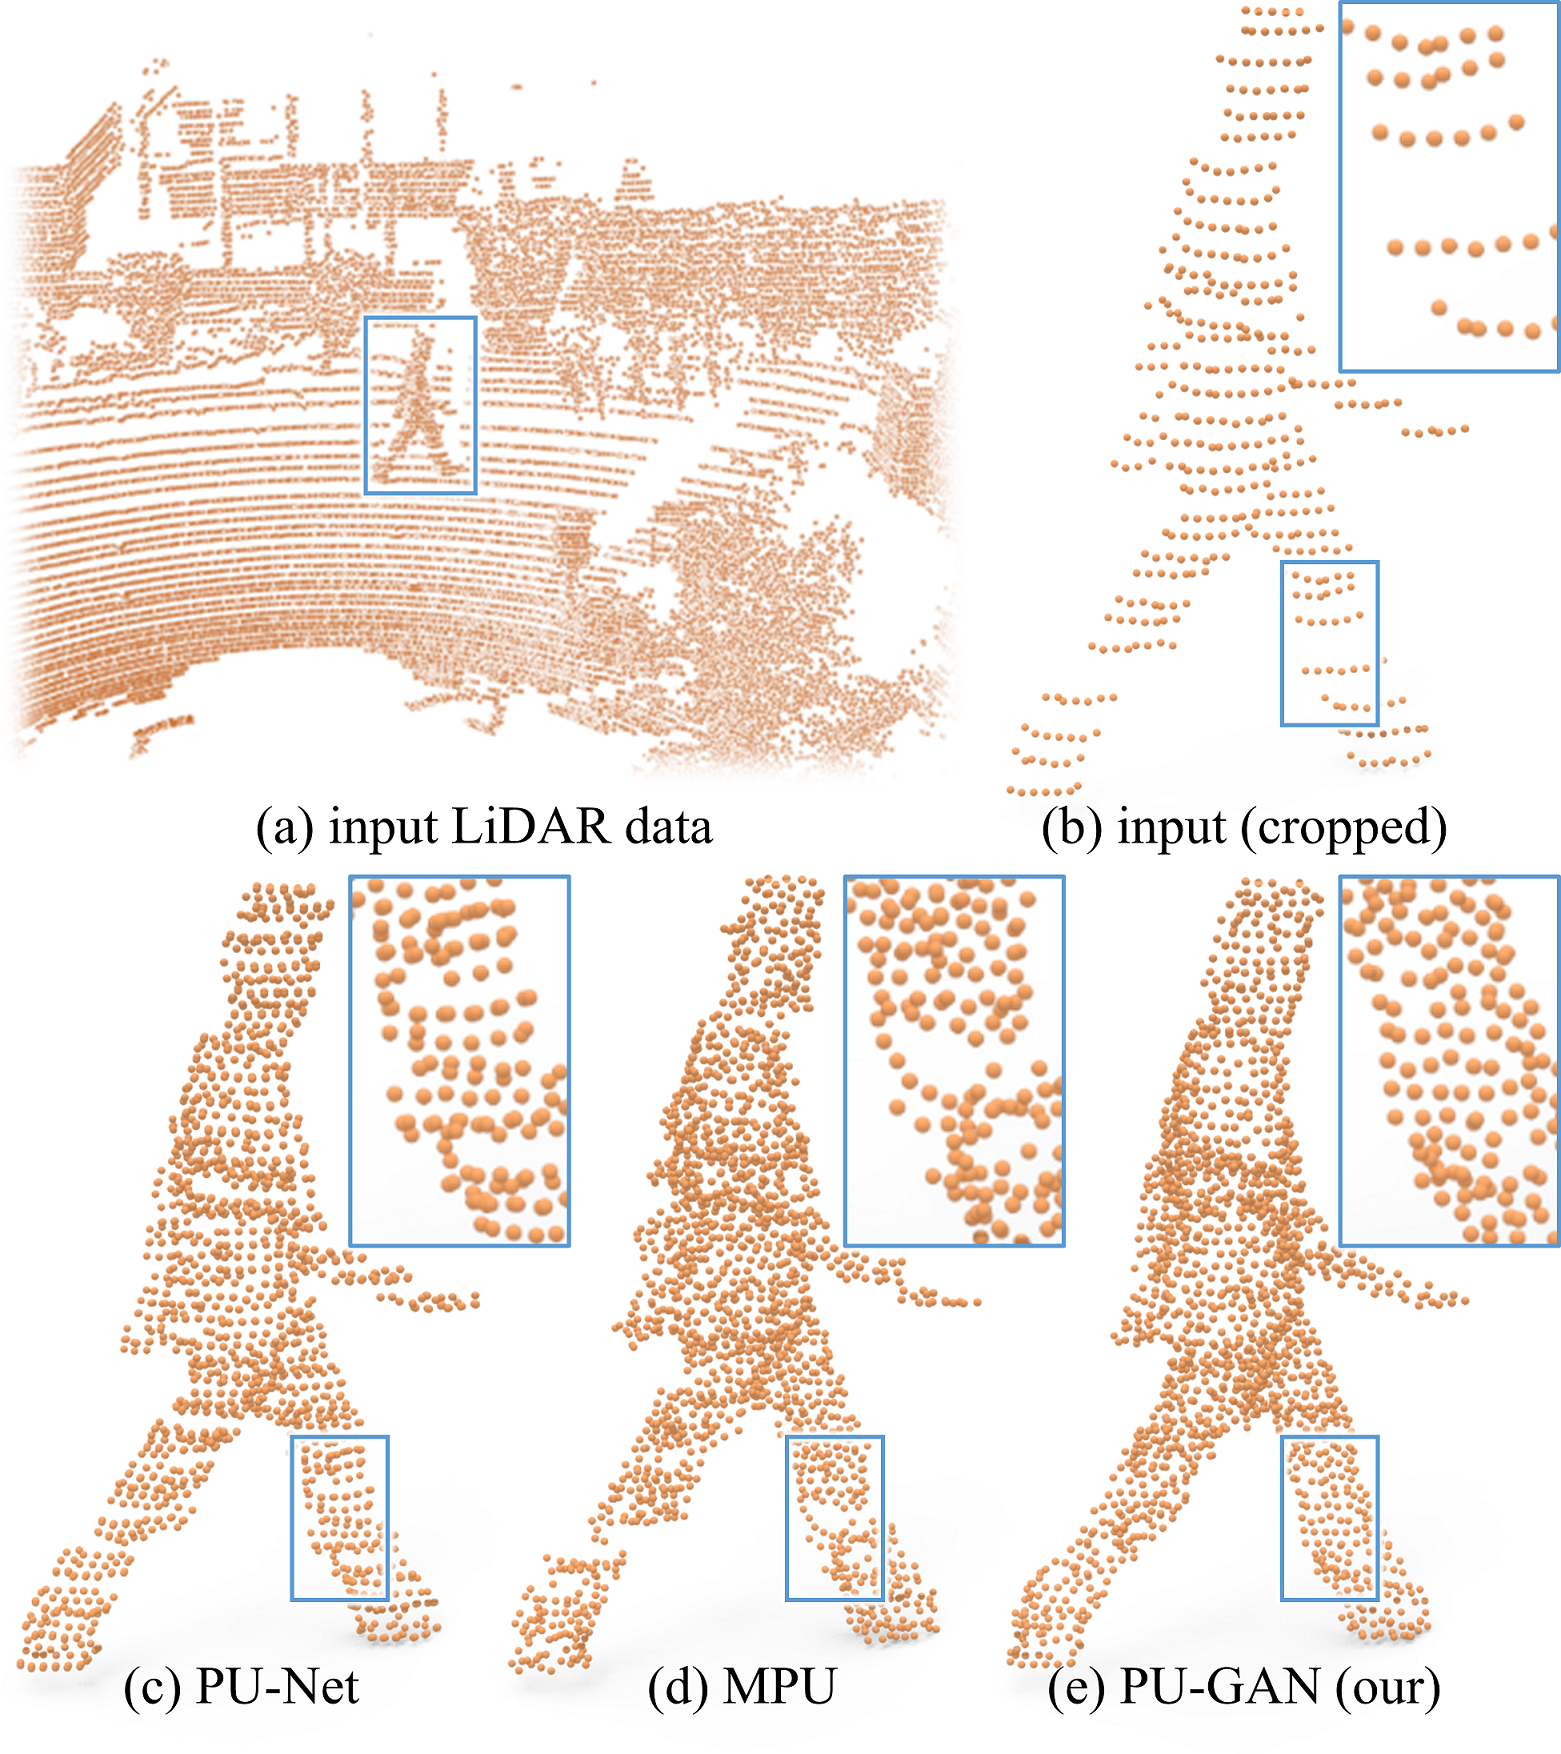
\includegraphics[width=0.95\linewidth]{teaser}
	\caption{Upsampling (b) a point set cropped from (a) the real-scanned KITTI dataset~\cite{geiger2013vision} by using (c) PU-Net~\cite{yu2018pu} (CVPR 2018), (d) MPU~\cite{yifan2018patch} (CVPR 2019), and (e) our PU-GAN.
%The input (b) is cropped from the real-scanned KITTI dataset~\cite{geiger2013vision}.
Note the distribution non-uniformity and sparsity in the input.}
%The input is cropped from a real-scanned LiDAR data, the KITTI dataset~\cite{geiger2013vision}.}
	\label{fig:teaser}
	\vspace*{-2mm}
\end{figure}

% definition of point cloud
%Point cloud is a popular means to represent and process 3D geometry, due to its compactness and generality, as well as due to the fact that it is a standard output from 3D scanning.
% with depth cameras and LiDARs sensors.
%\dc{I suggest the following instead of the above}
Point clouds are the standard outputs from 3D scanning.
In recent years, they are gaining more and more popularity as a compact representation for 3D data, and as an effective means for processing 3D geometry.
%
However, raw point clouds produced from depth cameras and LiDAR sensors are often sparse, noisy, and non-uniform.
This is evidenced in various public benchmark datasets, such as KITTI~\cite{geiger2013vision}, SUN RGB-D~\cite{song2015sun}, and ScanNet~\cite{dai2017scannet}.
Clearly, the raw data is required to be amended, before it can be effectively used for rendering, analysis, or general processing.

%good-quality point clouds without these issues are highly demanded by many applications like rendering, surface reconstruction, and object recognition.

%,~\eg, high-resolution surfel-based point set rendering, surface reconstruction, autonomous navigation, virtual reality,~\etc.
%
%\phil{XZ: please show these applications with comparison at the end of paper}

% definition of point cloud upsampling
%Currently, there are various public benchmarks on point clouds,~\eg, KITTI~\cite{Geiger2012CVPR}, SUN RGB-D~\cite{song2015sun}, ScanNet~\cite{dai2017scannet},~\etc.
%However, these point sets scanned by customer-level devices are typically sparse, noisy and incomplete.
%Thus, point cloud upsampling is particularly necessary.

Given a sparse, noisy, and non-uniform point cloud, our goal is to upsample it and generate a point cloud that is \emph{dense}, \emph{complete}, and \emph{uniform}, as a faithful representation of the underlying surface.
%, without small holes in the results.
%
These goals are very challenging to achieve, given such an imperfect input, since, apart from upsampling the data, we need to fill small holes and gaps in data, while improving the point distribution uniformity.
%; see Figure~\ref{fig:teaser}.
%
%Particularly, we
%\emph{uniformly} and \emph{completely} located on the underlying geometry.
%Different from shape completion, point cloud upsampling does not aim to reconstruct large missing parts and structures that are absent in the input, but it should have the ability to fill in small holes that are caused by the very sparse and non-uniform point distribution.
%However, it is quite challenging to meet the above requirements due to the unordered and irregular properties of 3D points.
%This upsampling problem is quite challenging because the generated dense points should not only describe the underlying geometry of a latent target object, but also have a uniform distribution and roughly cover the complete object surface.
%Hence, simply inserting new points between original points is insufficient.

% current methods and limitations
Early methods~\cite{alexa2003computing,lipman2007parameterization,huang2009consolidation,huang2013edge,wu2015deep} for the problem
%of upsampling and consolidating point clouds
are optimization-based, where various shape priors are used to constrain the point cloud generation.
%
Recently, deep neural networks brought the promise of data-driven approaches to the problem.
Network architectures, including PU-Net~\cite{yu2018pu}, EC-Net~\cite{yu2018ec}, and very recently, MPU~\cite{yifan2018patch}, have demonstrated the advantage of upsampling point clouds through learning.
%
%However, these networks may not be able to produce good results from low-quality inputs (particularly those acquired from real 3D scanning) that are sparse, noisy, and non-uniform; see Figure~\ref{fig:teaser} (c)-(e) for a comparison.
%\dc{I suggest a finer and more careful claim, instead of the above:}
%
However, these networks may not produce plausible results from low-quality inputs that are particularly sparse and non-uniform;
in Figure~\ref{fig:teaser} (c)-(e), we show a typical example that demonstrates the advantage of our method, which unlike the other networks, it combines completion and uniformity together with upsampling.

%generate a complete and uniform point cloud given a very non-uniform sparse point set as input; see Figure~\ref{fig:teaser} (b-c) as examples.

%Most of the existing methods upsample points by solving some kind of optimization, which is commonly constrained by the shape priors~\cite{alexa2003computing,lipman2007parameterization,huang2009consolidation,huang2013edge,wu2015deep}.
%These optimization-based methods, however, tend to yield poor performance when the priors or assumptions are not satisfied.
%Recently, deep learning brings the promise of the data-driven approach.
%Network architectures like PU-Net~\cite{yu2018pu}, EC-Net~\cite{yu2018ec}, and MPU~\cite{yifan2018patch} are successful at upsampling sparse points.
%However, these networks cannot generate a complete and uniform point cloud given a very non-uniform sparse point set as input; see Figure~\ref{fig:teaser} (b-c) as examples.

%\if 0
%% the success of GANs in the field of image processing
%Recently, the generative adversarial network (GAN) has shown its feasibility and capability for image super-resolution with %photo-realistic effect~\cite{ledig2017photo,wu2017srpgan,yuan2018unsupervised,wang2018fully}.
%The key to GAN's success is the idea of an adversarial loss that forces the generated images to be, in principle, %indistinguishable from real photos~\cite{zhu2017unpaired}.
%Naturally, also as a generation task, point cloud upsampling may benefit from such idea of GAN, since we can employ the %adversarial loss to force the generated points to have a uniform distribution.
%However, the adaption of GAN-based techniques to point cloud upsampling is far from straightforward.
%\fi

% our work
%In this work, we present a new point cloud upsampling framework, namely PU-GAN, based on the generative adversarial net (GAN).
%
In this work, we present a new point cloud upsampling framework, namely PU-GAN, that combines upsampling with data amendment capability.
The key contribution is an adversarial network to enable us to train a generator network to learn to produce a rich variety of point distributions from the latent space, and also a discriminator network to help implicitly evaluate the point sets produced from the generator against the latent point distribution.
Particularly, the adversarial learning strategy of the GAN framework can regularize the predictions from a global perspective and implicitly penalize outputs that deviate from the target.
%\phil{I avoided to talk too much about the loss and talk about bypassing the loss, since we also need a loss with several terms (may look complicated) in our method}


%that bypass the need to guide the reconstruction by carefully designed losses. Using a

%GAN framework enables training a generator network generating} a richer variety of point distributions from the latent space, as well as to train a discriminative network to implicitly evaluate the point sets produced from the generator against the true point set distribution. \dc{What is ``true''???}. ...against plausible examples that are dense, complete and have a uniform distribution.
%avoid the necessity of explicitly designing a loss function to guide the generation of point clouds, and on the other hand, to implicitly learn a rich variety of point distributions.
%Particularly, we sidestep the necessity of an explicit loss to directly guide the point set generation, since designing such a loss is hard for our problem, which aims not only for a dense and complete point set but also for a uniform point distribution.
%\dc{It is a bit of repetition, but never mind}
%Particularly, it is hard to design an ideal loss for our problem, where we aim not only for a dense and complete point cloud but also for the point distribution uniformity.
% without direct knowledge of the underlying distribution.

However, successfully training a working GAN framework is known to be challenging~\cite{goodfellow2014distinguishability,radford2015unsupervised}, particularly the difficulty to balance between the generator and discriminator and to avoid the tendency of poor convergence.
%converging to a poor model.
%
Thus, we first improve the point generation quality, or equivalently the feature expansion capability, of the generator, by constructing an up-down-up unit to expand point features by upsampling also their differences for self-correction.
Besides, we formulate a self-attention unit to enhance the feature integration quality.
Lastly, we further design a compound loss to train the network end-to-end with adversarial, uniform, and reconstruction terms to enhance the distribution uniformity of the results and encourage the discriminator to learn more latent patterns in the target distribution.


%
%In this work, we present a novel generative adversarial network (GAN) based framework for point cloud upsampling, namely PU-GAN.
%Compared with manually designing a loss to model the ``ideal'' distribution, we only need to provide ground truth exmaples and the GAN framework can learn multimodal structure of the target distribution, for which a simple variational approximation is infeasible.
%generate the dense points automatically without any priors or constraints.
%As shown in Figure~\ref{fig:teaser} (a), the input real-scanned LiDAR point cloud is very sparse and non-uniform.
%Even under such severe case, our PU-GAN still generates a dense result with complete and uniform point distribution; see Figure~\ref{fig:teaser} (d).

%However, the convergence of training GAN is still an open challenge~\cite{goodfellow2014distinguishability} since it is hard to balance the ablities of the generator and the discriminator during training.
%For instance, if the generator fails to learn the patterns of the target distribution, the discriminator can perfectly distinguish the generated distribution from the target~\cite{arjovsky2017towards}, thus leading to the complete stop of the training process.
%The discriminator must first transfer the new patterns to the generator and then the latter will generate more realistic samples to challenge the former.
%Hence, to make the GAN framework feasible and capable for this upsampling task, we further introduce the following adaptations.
%First, we introduce a novel uniform loss to improve the uniformity of the generated distribution.
%This can promote the training of the discriminator.
%Second, to enhance the feature embedding ability of both generator and discriminator, we further present an up-and-down unit for %error feedback and self-correcting, as well as a self-attention module.
%Last but not least, we merge the farthest sampling into the generator to make the generated points more uniform.

To evaluate the upsampling quality of PU-GAN, we employ four metrics to assess its performance against the state-of-the-arts on a variety of synthetic and real-scanned data.
Extensive experimental results show that our method outperforms others in terms of distribution uniformity, proximity-to-surface, and 3D reconstruction quality.

%To demonstrate the quality of upsampling results, we employ four evaluation metrics to assess the performance of our PU-GAN against the state-of-the-arts using a variety of synthetic and real-scanned data.
%The extensive experiments show that our method outperforms others in terms of distribution uniformity, proximity-to-surface, and 3D reconstruction quality.
%The extensive experiments show that our method compares favorably with others and particularly, the results generated by our PU-GAN are more uniform both locally and globally.

%Specifically, we employ the generator to consume sparse points as input and produce a dense point set (or fake point set).
%We then feed the fake point set into the discriminator to determine if it has the same uniform distribution as the ground truth.
%Note that we consider the points generated by Poisson disk sampling algorithm as the ground truth, since such point distribution has blue noise pattern and is generally considered ideal for many applications~\cite{cook1986stochastic}.

\if 0
Overall, our contributions are summarized below:
\begin{itemize}
	\item
	To the best of our knowledge, we are the first to propose a GAN-based point cloud upsampling network.
	\item
	We propose a series of adaptations for network architecture, including an up-and-down unit with error feedback mechanism, a self-attention module for feature extraction, and the insertion of the farthest sampling into the network structure.
	\item
	We introduce a joint loss function for end-to-end training. Particularly, we propose a novel uniform loss to encourage the upsampled points with a uniform distribution.
\end{itemize}
\fi

